\chapter{Experimenton and Results}

\section{Introduction}
With the configuration described in the previous section we can now start to experiment with the robotic platform to do certain navigation tasks. In this part we propose various experiments that try to evaluate the  performance of the \ac{FMCW} \ac{RADAR} as an alternative or support to the \ac{LiDAR} as an obstacle detector for indoor navigation.
\section{Obstacle Avoidance}
Over the course of this work it was concluded that the radar data was not appropriate for Map Building or for localization using \ac{AMCL}. However it was noted that the radar was quicker at perceiving effective at detecting different types of obstacles. 


There are two ways in which the navigation stack deals with obstacle avoidance. One way is to plan around the obstacle using the global planner if the obstacle is said on the .
The motion controller will take into account this plan 


\section {Experiment 2}
In this following test we want to answer two things: (1) Is the robot able to avoid people that obstruct its pre planned path only using the  \ac{FMCW} radar as an obstacle detector, and (2) if in this case it is also able to clear previously obstructed spaces (by the person in this case) by raytracing its environment. This last requirement may provide to be difficult to get since the radar point cloud is less dense than the 2D laser range finder.
\subsection{Experimental Setup}
The robot starting position and goal were set the same as the last test, however in this case a single person was instructed to actively obstruct the robot's forward movement until the robot reaches its first goal. After reaching it the person is removed from the environment  and the robot is  instantaneously given a second goal which in this case is its the starting position. 
\subsubsection{Results}
\subsubsection{Laser}
As expected the robot was able to detect and avoid the person in all 5 cases. However it should be noted that in one of this cases the robot tried to avoid it by going through an obstructed space due to a missed detection. This lead to collision. The robot was also able to clear the previously obstructed spaces, getting to the starting position without avoiding past marked obstacles.
\subsection{Radar}
The radar was also able to detect the obstructing person and managed to plan around it in all cases. Since the radar cloud is less dense, clearing marked obstacles was slower than in the \ac{LiDAR} case. However this did not impact the overall performance of the navigation task in a significant way since it still had 
\subsection{Comments}
 The radar was also able to perform 
obstacle avoidance of dynamic obstacles (in this case a person that continuously obstructed its path at 5 different times in the same environment which may suggest the use of \ac{RADAR} as an alternate sensory unit over the \ac{LiDAR}.
\section {Experiment 3}
Over the course of this work the \ac{FMCW} radar has shown to have better performance at detecting certain indoor objects than the 2D \ac{LiDAR}. This means that there might be situations where using the \ac{FMCW} radar for obstacle avoidance produce better results for indoor navigation tasks. To demonstrate this a test was devised in a controlled environment that compares the performance of each sensor for different types of obstacles, in this case two types of chairs, a garbage bin, a low height box and finally a robot (in this case another tutlebot2).  We also try to use the fusion of both sensors that in theory should produce the best results.


To ensure the experiment is done in a controlled way the scenario in figure X was constructed. This is a 4 by 4 meter squared box with 1 meter walls with the addition of a half a meter wall in length in the middle. This type of environment optimizes the robots localization system (\ac{AMCL}) as well as make sure we only concentrate with one specific object at a time. Using a \ac{SLAM} package developed here at \ac{IRIS} a map is created (Figure X) that will later be used for localization purposes.
\subsection{Experimental setup}
With the described scenario we setup the robots goal to make 5 loops between 2 goals, positioning in between the route an obstacle as described in  figure X. If the obstacle detection system fails then the robot should collide with said object, if it succeeds the robot should go around the object leaving in between a relatively safe distance. The test was made using the \ac{FMCW} radar, the 2D \ac{LiDAR}, and the fusion of both for different types of objects described in figure X. The  navigation data was recorded in a rosbag file in order to be analyzed later.

The list of objects are shown bellow:
%LIST
The first obstacle chosen is an office chair used here at \ac{IRIS} Laboratory (Figure X). This type of swivel chair has a load bearing leg under the seat  that  spreads into a set of wheels for mobility. The space this chair occupies is approximately a circle with 35 cm radius.
\subsection{Results}
In this section we show the results of how the robot performed in avoiding the previous obstacles using different type of sensor sources (\ac{FMCW} radar, the 2D \ac{LiDAR} and both).
\subsubsection{Office Chair}
In the \ac{LiDAR}'s case  the robot completely disregarded the chair going in a straight line and pushing it until it was away from the experimental setup has shown in the video X. This was due to the 2D \ac{LiDAR} only detecting the leg of the chair and not the wheels. This means that the robot only perceived a single point as being occupied and not the full area of the chair. Although the inflation layer  might correct this error in some cases, since the detection is so late the robot still is unable to avoid it.

However with the \ac{FMCW} radar the chair is detected almost immediately, this makes the global planner and motion controller to be able to adjust in a very comfortable way and with it the robot is able to avoid collision. Figure X shows some instances of the first experiment. Although the detected space that the chair is occupying has some mismatch, the early detection makes up for it. However since the radar has small field of view (120 degrees) the robot might not detect the obstacle when it is passing by it which in this case lead to it scraping by the chair one time.
\subsubsection{Normal Chair}
As shown in figure X and in video y the robot did not perform optimally using \ac{LiDAR}. First off it went in a straight line just as the previous case almost hitting  the legs of the chair. However when it got to close to it, it came to a halt and kept oscillating for a long time until it either collided with the leg or scrapping by it. This was again was due to the \ac{LiDAR} only detecting the obstacles at small distances. This behavior repeated itself throughout the task, leading to the chair being pushed several times. 

Using the \ac{FMCW} radar proved to be much better with the robot safely circumventing around the chair with safe distance for all duration of the task. Analysing the data we see that when the robot is facing it it detects almost all legs immediately (Fig X). This makes it so the robot is aware of it at all times and planning around it.
\begin{figure}[h] 
\centerline{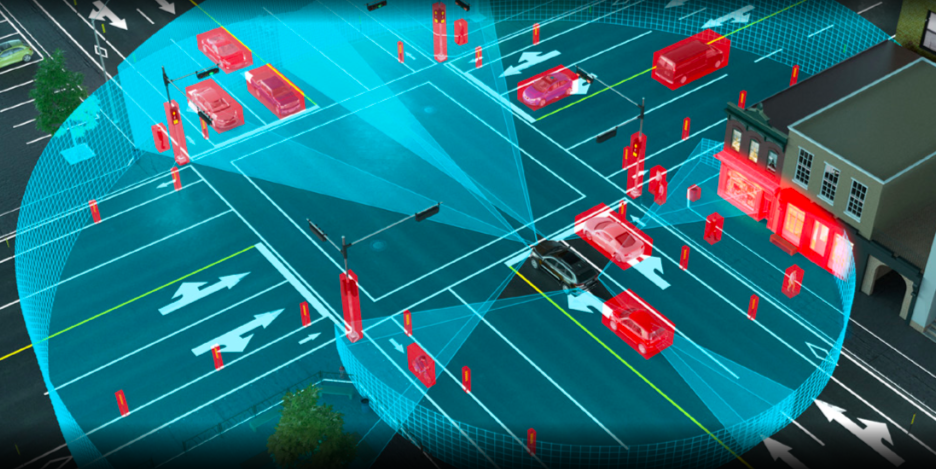
\includegraphics [width=0.7 \textwidth]{imgs/chapter/lidarcar.png}}
\caption{Trajectory of the robot using the office chair as an obstacle}
\label{fig:lidarcar}
\end{figure}

\subsubsection{Garbage Bin}
The robot went in a straight line as in the wheeled chair's case pushing the garbage bin until it reached its first goal. This happened again because the \ac{LiDAR} was unable to detect the garbage bin. Using the \ac{FMCW} radar the robot did detect it properly and went around it easily.
\subsubsection{Box}
Collided with the chairs multiple times and 
\subsubsection{Robot}
Both \ac{LiDAR} and the FMCW radar were able to avoid the robot. 
In the wheeled chairs case the robot was able to detect 
- Image of plots
- explain what happened
- explain some navigation stack stuff

\section {Experiment 4}